\section{GPU-enabled parallel Schr\"odinger simulations}
\label{sec:3D Stirap parallel Schr\"odinger simulations}
For performance metrics, I will discuss the use of a GPU-enabled Schr\"odinger equation integrator developed by myself, based on and compared with the results to a multi-core MPI enabled version by T. Morgan and N. Crowley. We solved the Schr\"odinger equation for a fully three-dimensional potential, demonstrating its effectiveness and improved performance compared to standard HPC methods.

The problem we examined was that of a realistic system for coherent atomic control. Controlling the centre-of-mass movement of atoms between adjacent trapping potentials via adiabatic techniques, collectively known as \textit{spatial adiabatic passage} (SAP), has recently become a popular topic of investigation [cite review]. The STIRAP process [cite] is a widely studied and used optical technique for controlled state transfer, with an analogous effect in atom-optical systems. Herein I describe the motivation, physical system, and the numerical implementation for solution of this problem.

\subsection{Spatial adiabatic passage}

Significant work and progress has been made for control of the internal degrees of freedom of atoms. External degrees of freedom are, however, only recently being made realisable. The use of adiabatic techniques such as the SAP family of methods are very promising tools for high fidelity state generation. One such technique from this family is known as {\textit matter-wave STIRAP}[cite], which can be used for high fidelity atomic centre-of-mass control \cite{Eckert:04}. This method is used to transfer atomic population between trapping potentials and is highly robust to variation in the system parameters. The use of this technique has recently become experimentally accessible [private communication with S.~Taei from group of Y.~Takahashi], although many accessible systems have been proposed \cite{Eckert:06,Morgan:11,Kohler:13,Morgan:13}.

If we initially consider two separated harmonic potentials, with groundstates given by $| L \rangle$ and $| R \rangle$, a reduction of the distance between the traps increases the coupling, and hence tunneling rate, between them. This is modeled with the two-level Hamiltonian as
\begin{equation}
    H = -\hbar
    \begin{pmatrix}
        0 & \Omega_{LR} \\
        \Omega_{RL} & \Delta
    \end{pmatrix}
\end{equation}
where $\Omega_{LR} = \Omega_{RL}$ are the couplings between states, and $\Delta$ is the detuning of state $| R \rangle$, relative to $| L \rangle$. Assuming an atom initially localised in $| L \rangle$, and with an increase in coupling strength between the levels, the localised atom will tunnel from the $| L \rangle$ to $| R \rangle $. However, this processes is difficult to control, as Rabi oscillations introduce an explicit time-dependence and cause the atomic population to continuously transfer between both traps. This will require precise timing and control to ensure a fully robust transfer of population. Thus, a double-well potential is a difficult system in which to realise coherent control.

A more robust method, using three adjacent harmonic traps and the aforementioned matter-wave STIRAP process, improves upon the double-well system. For this SAP technique, we model the adjacent trapping potentials as coupled by their nearest neighbour solely. A model of this system for potentials $L,M,R$ on resonance, is given by the Hamiltonian
\begin{equation}\label{eqn:sap_ham}
    H = -\frac{\hbar}{2}
    \begin{pmatrix}
        0 & \Omega_{LM} & 0 \\
        \Omega_{LM} & 0 & \Omega_{MR} \\
        0 & \Omega_{MR} & 0
    \end{pmatrix},
\end{equation}
where $\Omega_{LM},~\Omega_{MR}$ describe the coupling between left-middle and middle-right potentials respectively. Diagonalising this Hamiltonian gives three distinctive eigenstates, however only one is of interest here. For the $\lambda=0$ eigenstate of this Hamiltonian, known as the \textit{dark state}, the dependence on the middle potential vanishes, with the state given by
\begin{equation}
 | 0 \rangle = \cos\ \Theta| L \rangle - \sin \Theta | R \rangle
\end{equation}
where $\Theta=J_{MR}/J_{LM}$ is the mixing angle. From the adiabatic theorem of quantum mechanics, it is known that if an eigenstate has its Hamiltonian perturbed slowly enough, then we can follow its evolution ensuring that it always remains in an eigenstate of the Hamiltonian. Thus, by preparing the system in state $| L \rangle$, and varying $\Theta$ slowly, we can shift the population from the leftmost harmonic potential to the rightmost, without populating the center.

\begin{figure}
    \centering
    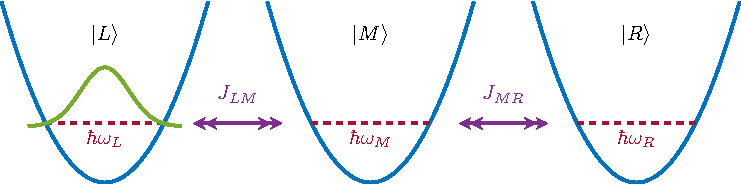
\includegraphics[width=0.75\textwidth]{./ch3_numerics/3potentials}
    \caption{Three trapping potential model for matter-wave STIRAP. The atom (green) is initially localised in the leftmost potential, $|L\rangle$, with the couplings between adjacent traps controlled by varying the distance dependent parameters $J_{LM},J_{MR}$.}
    \label{fig:ch3_stirap}
\end{figure}

This technique makes use of tunneling, with the rate of transfer between trapping potentials controlled by the respective spatial separation, and is demonstrated by Fig.~\ref{fig:ch3_stirap}. Typically, the method would be performed with time-dependent potentials. However, a static potential variant can be considered using parallel atomic waveguides, wherein the separation varies as a function of distance along the parallel axis. If we consider an atom that travels along such a waveguide, the coupling and hence tunneling rates seen by the atom in the waveguide are altered as the atom propagates. Such work has been discussed and considered in a realistic system for two spatial dimensions \cite{OSullivan:10}. Although a two dimensional model will be effective at describing much of the relevant dynamics, the lack of $z$-dimension ensures the effects stemming from dispersion, curvature of the waveguides and the absence of any such eigenstates along $z$ reduce the realism of such a model.



Thus, the goal of this project was to develop a realistic system for controlled movement of atoms with high fidelity amongst trapping potentials. The atomic population transfer between traps is controlled by the tunneling rate, through variation of the spatial separation between adjacent traps. It is instructive to note the counter-intuitive change of couplings between these potentials. For an atom initially located in the left potential, we increase $J_{MR}$ for the empty middle and right traps, before reducing again and increasing $J_{LM}$ for the left and middle. This is in direct contrast with a direct tunneling scheme, for which we directly increase the coupling between the populated left and empty middle, followed by middle and right. However, the direct scheme can be seen as two distinct combinations of the double-well case, and so carries the same time-dependent Rabi-oscillations. Comparing both methods will be instructive in discussing the advantages of the SAP routine over direct tunneling. %I will first discuss the physical model of this system.


\subsection{Physical model}

As discussed previously, to fully understand the dynamics of such a system we must investigate the fully three-dimensional model. One method of creating the required potential landscape is through the use of atom chips \cite{Bartenstein_ieee_2000}[cite Atoms and Wires: Toward Atom Chips]. These systems consist of micro-fabricated current-carrying wires, and can be used to create a variety of trapping potential shapes. With the application of current a magnetic field is created around individual wire, of which has a minima at the wire core. By applying an additional field orthogonal to the direction of current, this minima can be raised to a location above the wire surface, and can behave as a trapping potential for atoms, with an aditional field applied to prevent Majorana losses in the trap. Spatial and temporal adjustments of the potentials are possible, with a fine degree of control. These have been used extensively in recent years for trapping potentials [cite], and as atomic manipulators [cite].

For this work, the system was modeled as three adjacent wires on the atom-chip surface. By applying current and the appropriate magnetic fields to these wires, magnetic minima would be created to act as atomic waveguides. To avoid dispersion, and ensure the atom moved along the waveguide, a harmonic oscillator potential was also added along the parallel axis. The process of simulating the system involved localising the atom by a barrier at one end of the $|L\rangle$ potential, with the system evolved in imaginary time to find the groundstate. After finding the the groundstate, the barrier was removed, and the atom was allowed to propagate along the length of the waveguide. The populations in each waveguide could be tracked and calculated at each step of the process, with the final populations taken as the atom approached the end of the harmonic oscillator. The fidelity of the process could then be calculated by comparing the initial $| L \rangle$ and final $|R \rangle$ populations, as well as any intermediary $| M \rangle$ populations. Thus, to fully examine all such dynamics of the system, it is essential to investigate a fully three-dimensional model, which can take into account non-idealised real-world parameters.

Given that fully three-dimensional simulations of the Schr\"odinger equation are numerically expensive, the use of GPU computing methods are an ideal candidate for accelerating the simulation \cite{Bauke:11}. I will now discuss the resulting data and metadata of the simulations.



%%


\subsubsection{GPU computing performance}

%As fully three-dimensional simulations of the Schrodinger equation are challenging numerically, the use of GPU computing is an effective way to overcome many of the barriers. Whereas traditional computers perform computations using the central processing unit (CPU), GPU computing allows some of the work to be offloaded to the graphics processor.
As discussed in Section \ref{gpu section}, one example where GPGPU computing offer large performance gains are fast Fourier transformations (FFTs), with the Fourier split operator method being an ideal candidate for GPU systems \cite{Bauke:11}. The body of work for implementing this algorithm was using C, CUDA and Nvidia's CUFFT libraries for the Fourier transforms, whereas the MPI-enabled code similarly, was implemented using C.

To demonstrate the performance offered by GPU computing we compared it to using FFTW with MPI, a well used parallel programming paradigm and library. The message passing interface (MPI) implementation allows the code to be run across multiple machines, benefiting from the parallelism which may be offered by a supercomputing cluster. Although MPI-enabled FFTW is fast and supports extremely large grid sizes, it requires cluster access of a significant size to be a viable option. The MPI work on this project was carried out on the ICHEC system Stoney over the period 2010 to 2011, with all performance metrics data calculated therefrom.



Due to the hardware limited memory on the GPU, and that the dynamics along the $x-z$ plane were of most importance, the grid-size of the simulations were scaled as $256\times 64\times1024$ ($x\times y\times z$). Of next importance was the timestep of the simulation.  To ensure minimal loss in precision, the timestep of the simulations were chosen as $\Delta t = 1\times 10^{-6}$ s. For the GPU simulations, the test system was an Intel Core i7 2600K CPU at stock frequency, 8GB DDR3 memory operating at 1600 MHz, 7200 RPM HDD, Nvidia GeForce GTX 580 with 3GB of onboard memory running at 783 MHz GPU core frequency, 1566 MHz shader processor frequency, and 2010 MHz memory frequency. For all simulations the desktop was running Ubuntu 11.10 64-bit operating system and all calculations were performed in double precision (64-bit floating point) where applicable.

Table \ref{tbl:timing} shows the approximate timings for the completion of runs on GPU and CPU. Not only does GPU computing offer a 6-fold improvement over a single CPU, it also allows us to achieve a performance level which is comparable to an 8-node 8-core (64 cores) core MPI enabled CPU calculation. For a modest choice of GPU this offers substantial performance gains.

\begin{table}[tb]
  \begin{center}
    \begin{tabular}{|c||c|c|c|}
      \hline
      Device & Num. Devices & Timing  & Rel. Improvement \\ \hline
      CPU (MPI) & 8 & $\sim$6 Hr & 1.0$\times$ \\
      & 16 & $\sim$4 Hr & 1.5$\times$ \\
      & 32 & $\sim$1.5 Hr & 4.0$\times$ \\
      & 64 & $\sim$1 Hr & 6.0$\times$ \\ \hline
      GPU & 1 & $\sim$1 Hr & 6.0$\times$ \\ \hline
    \end{tabular}
  \end{center}
   \caption{The approximate times taken to simulate the propagation of an atom through our atom chip system on both GPU and CPU.}
   \label{tbl:timing}
\end{table}



\subsection{3D Simulations}
\label{sec:Results}

Given the large parameter space over which this system could be optimised, many simulations were required to determine optimal system behaviour. Making use of eight Nvidia M2090 GPUs available at OIST, terabytes of numerical results were generated in a relatively short time. The simulations assumed a single $^{6}$Li atom localised in the left waveguide. Its transversal wavefunction was determined numerically, with the assumption of a longitudinal Gaussian profile of similar width. The atom was then allowed to propagate along the waveguide potential, with the tunneling region at the centre of the chip.

The simulations allowed the verification of the addition of the magnetic fields at the center of the atomchips, which in turn drives the central potential out of resonance with the outer two. By adjusting the current in the central wire, such that the magnetic minima was in resonance only within the tunneling region allowed the matter-wave STIRAP process to work as expected. The resulting potentials for equal and optimal currents are given by Fig.~\ref{fig:equaloptcurrent}, showing a slice along $x-z$ and $x-y$ planes for both cases.

The populations for both the direct tunneling case, and matter-wave STIRAP processes are shown in Fig.~\ref{mwsVsDT}, with the wavefunction probablity density in the tunneling region given in Fig.~\ref{mwsVsDT}. The direct tuneling case can be seen to show large Rabi oscillations across the potentials, with the MWS process showing a much cleaner transfer, with minimal occupation of the central potential.

\begin{figure}[tb]
    \centering
  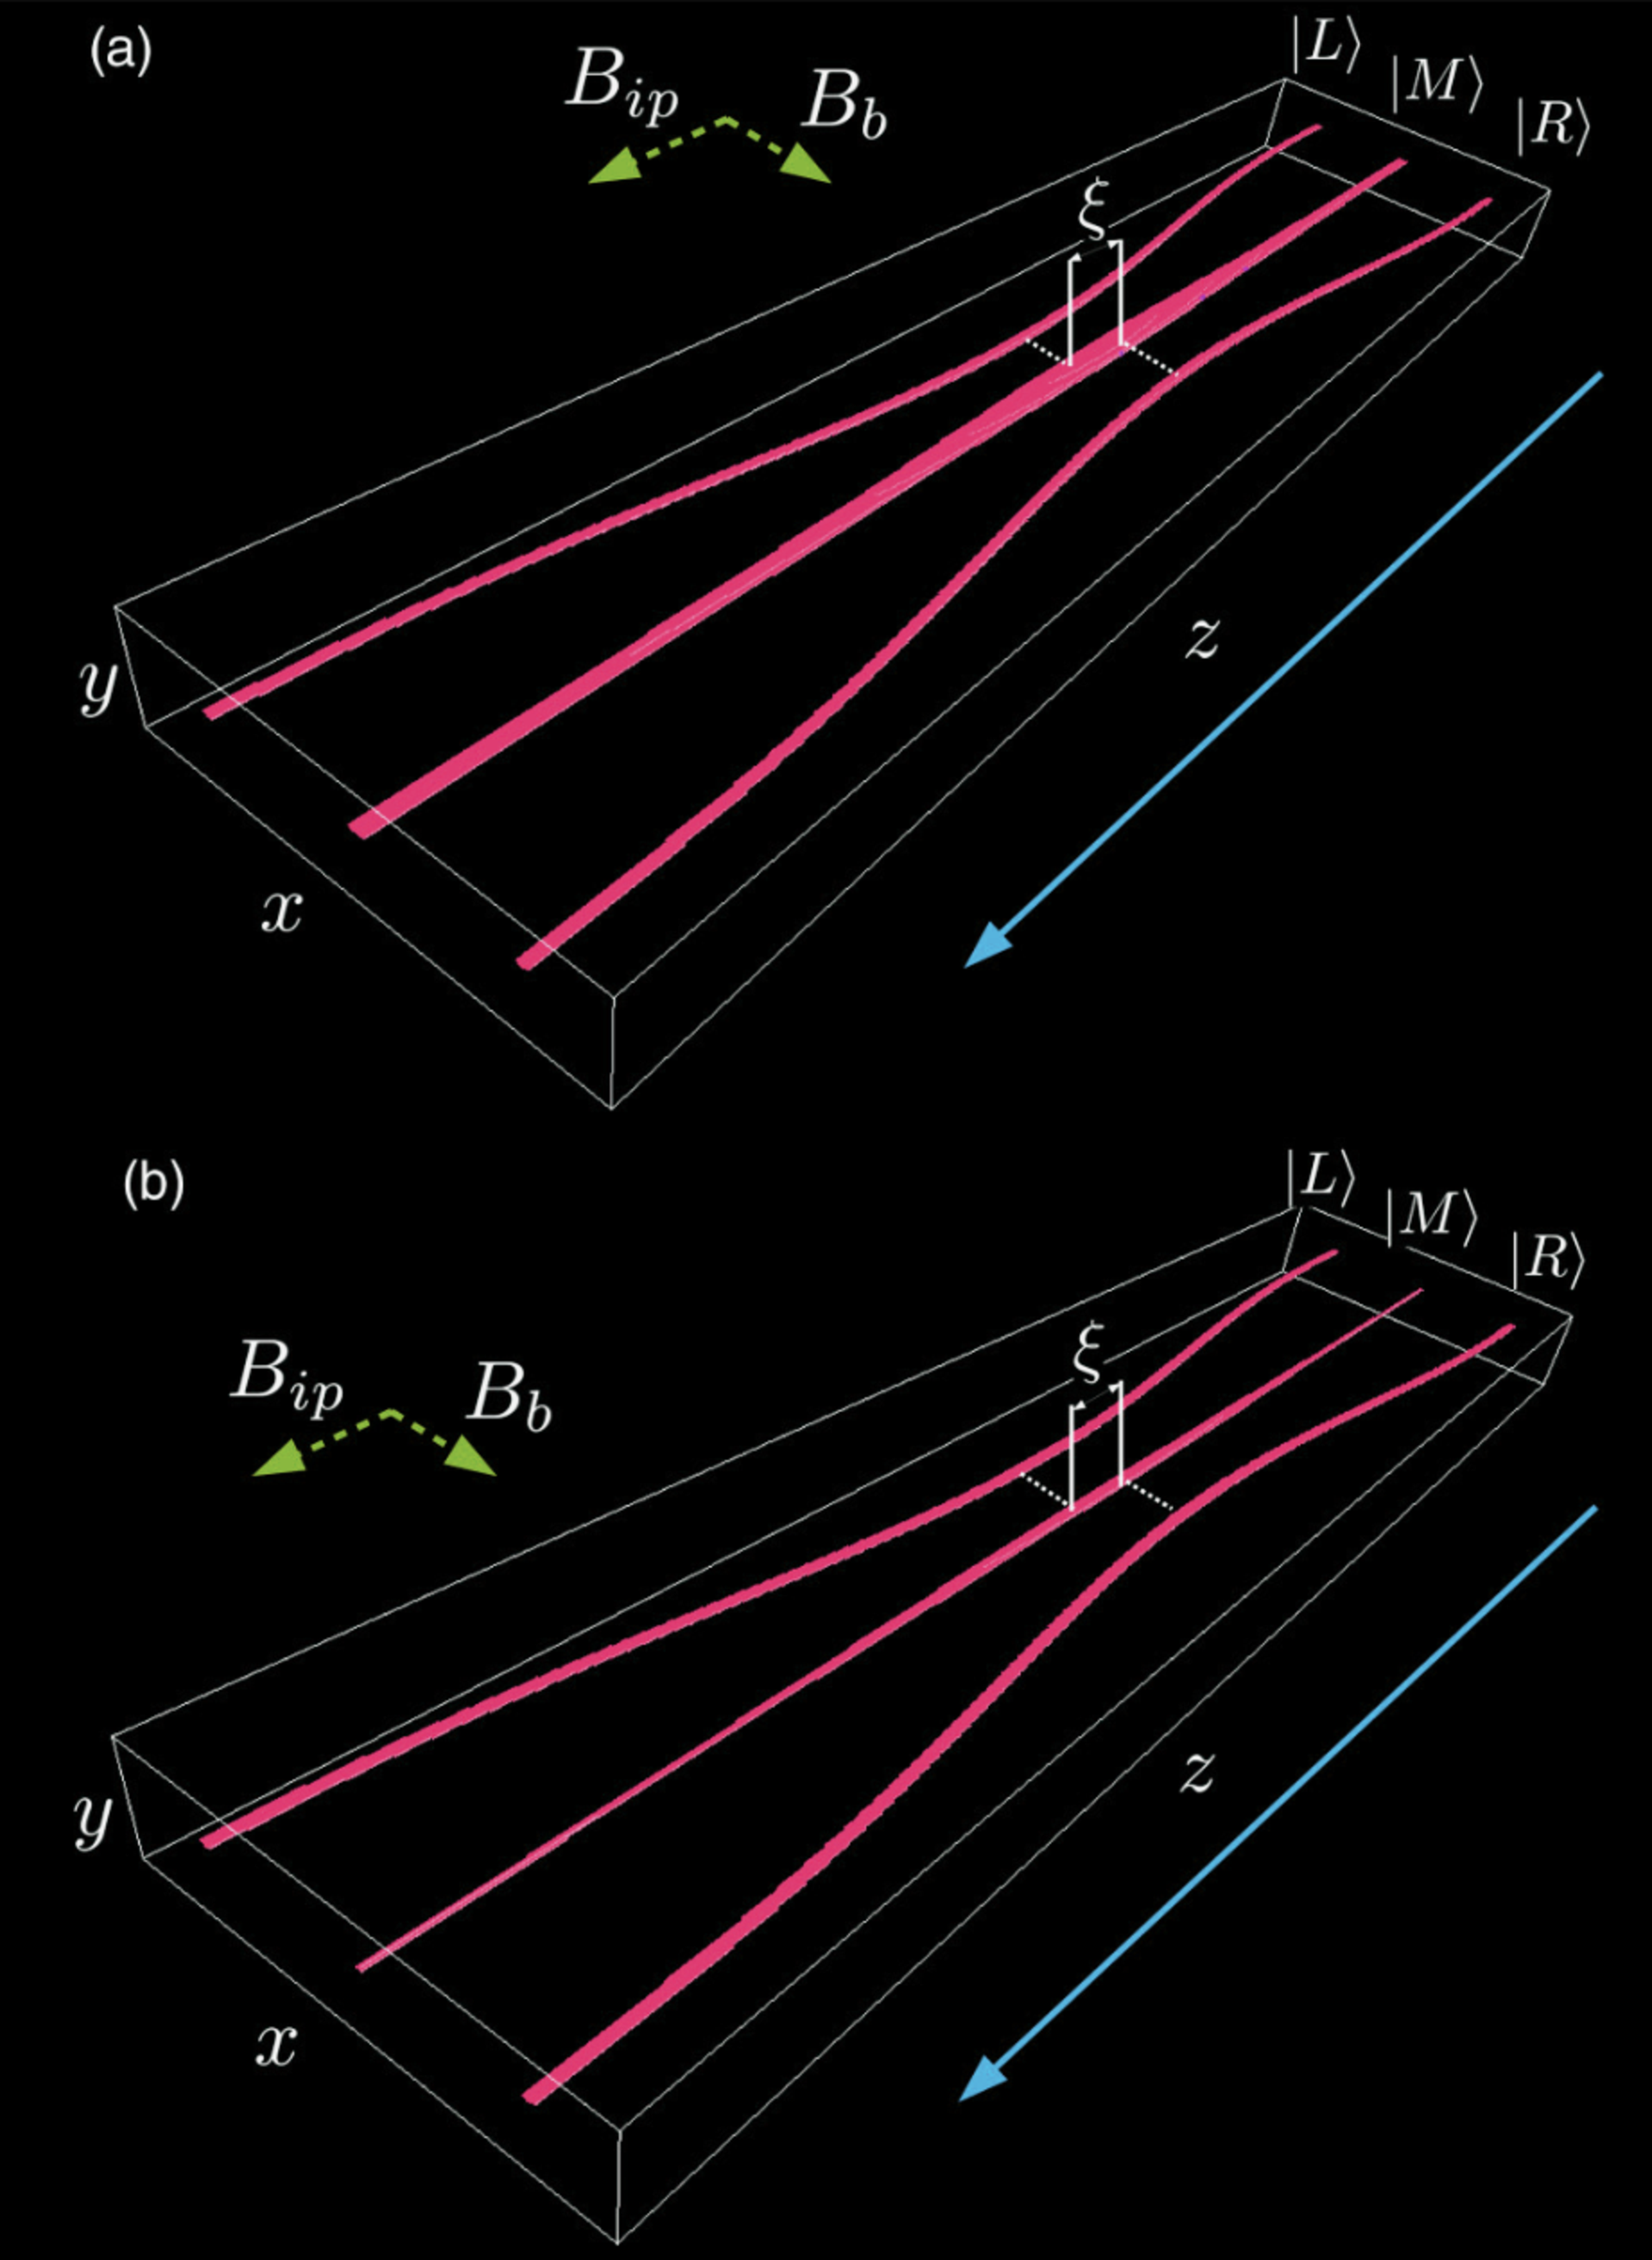
\includegraphics[width=0.85\textwidth]{ch3_numerics/3dpot.pdf}
  \caption{3d}
  \label{fig:Populations}
\end{figure}

\begin{figure}[tb]
    \centering
  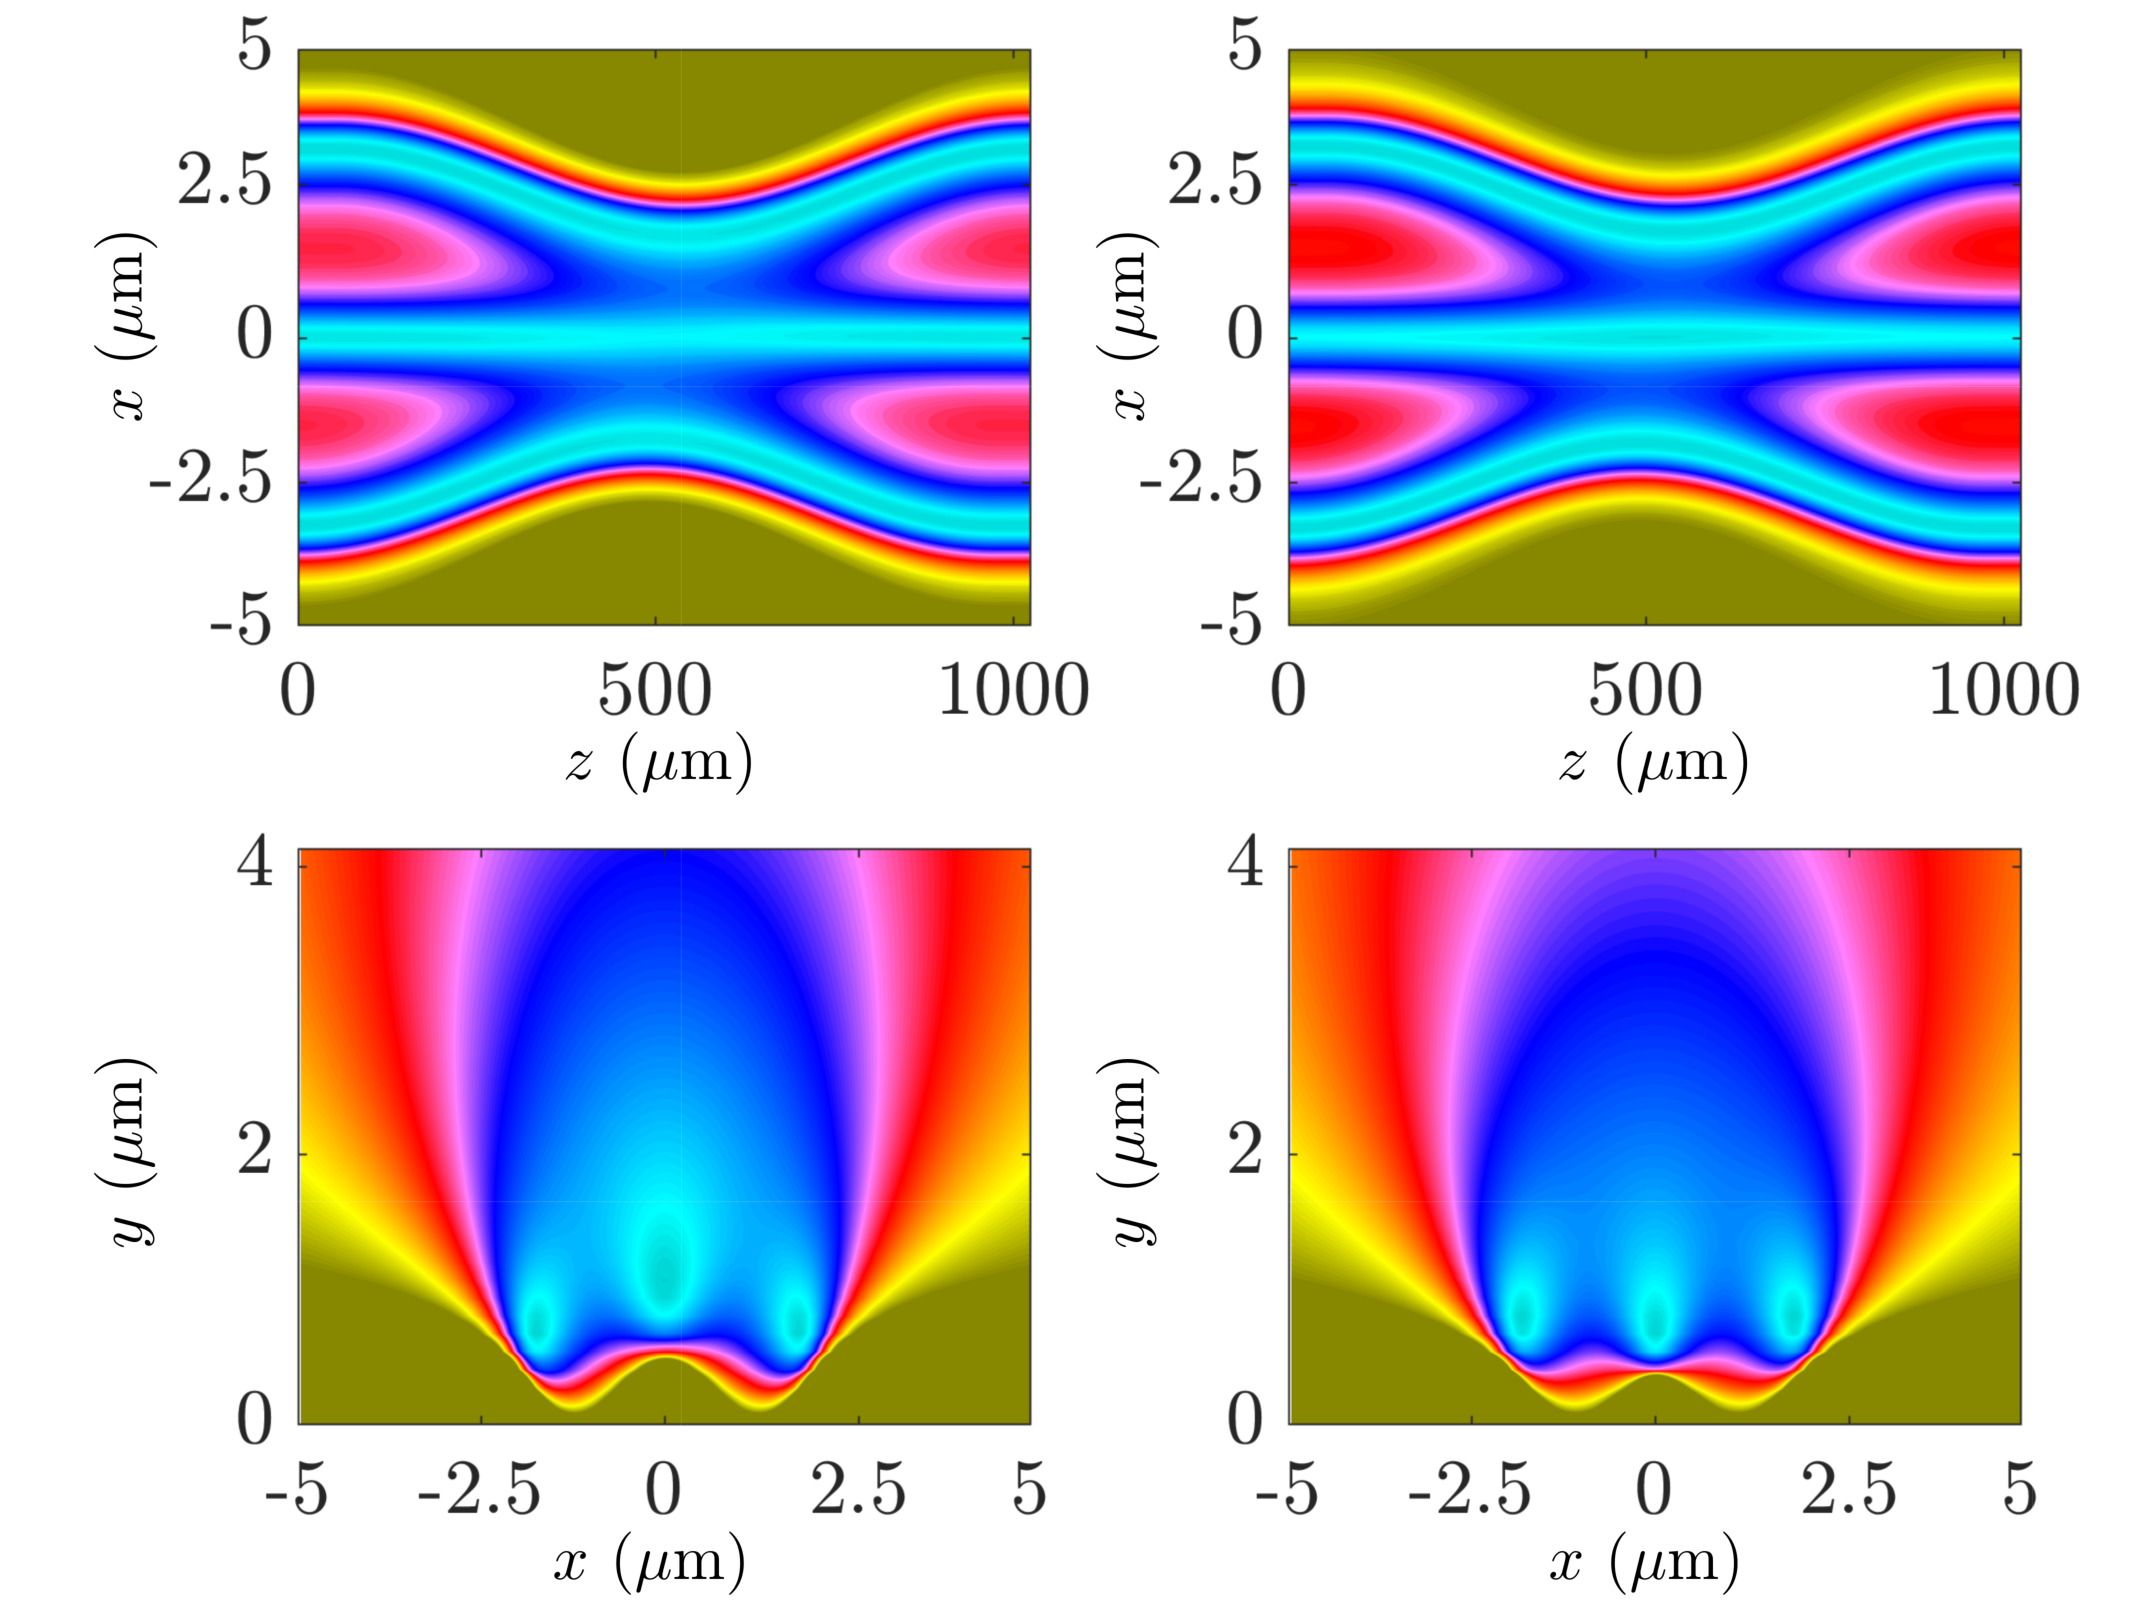
\includegraphics[width=0.85\textwidth]{ch3_numerics/potentials2.pdf}
  \caption{(Color online) The population in the left (blue dashed line), middle (green dot-dash line) and right (red solid line) waveguides as a function of time for (a) the counter-intuitive waveguide arrangement and (b) for intuitive, direct tunnelling one. The current in the middle wire is reduced to $I_M=0.07 A$.}
  \label{fig:Populations}
\end{figure}

\begin{figure}[tb]
    \centering
  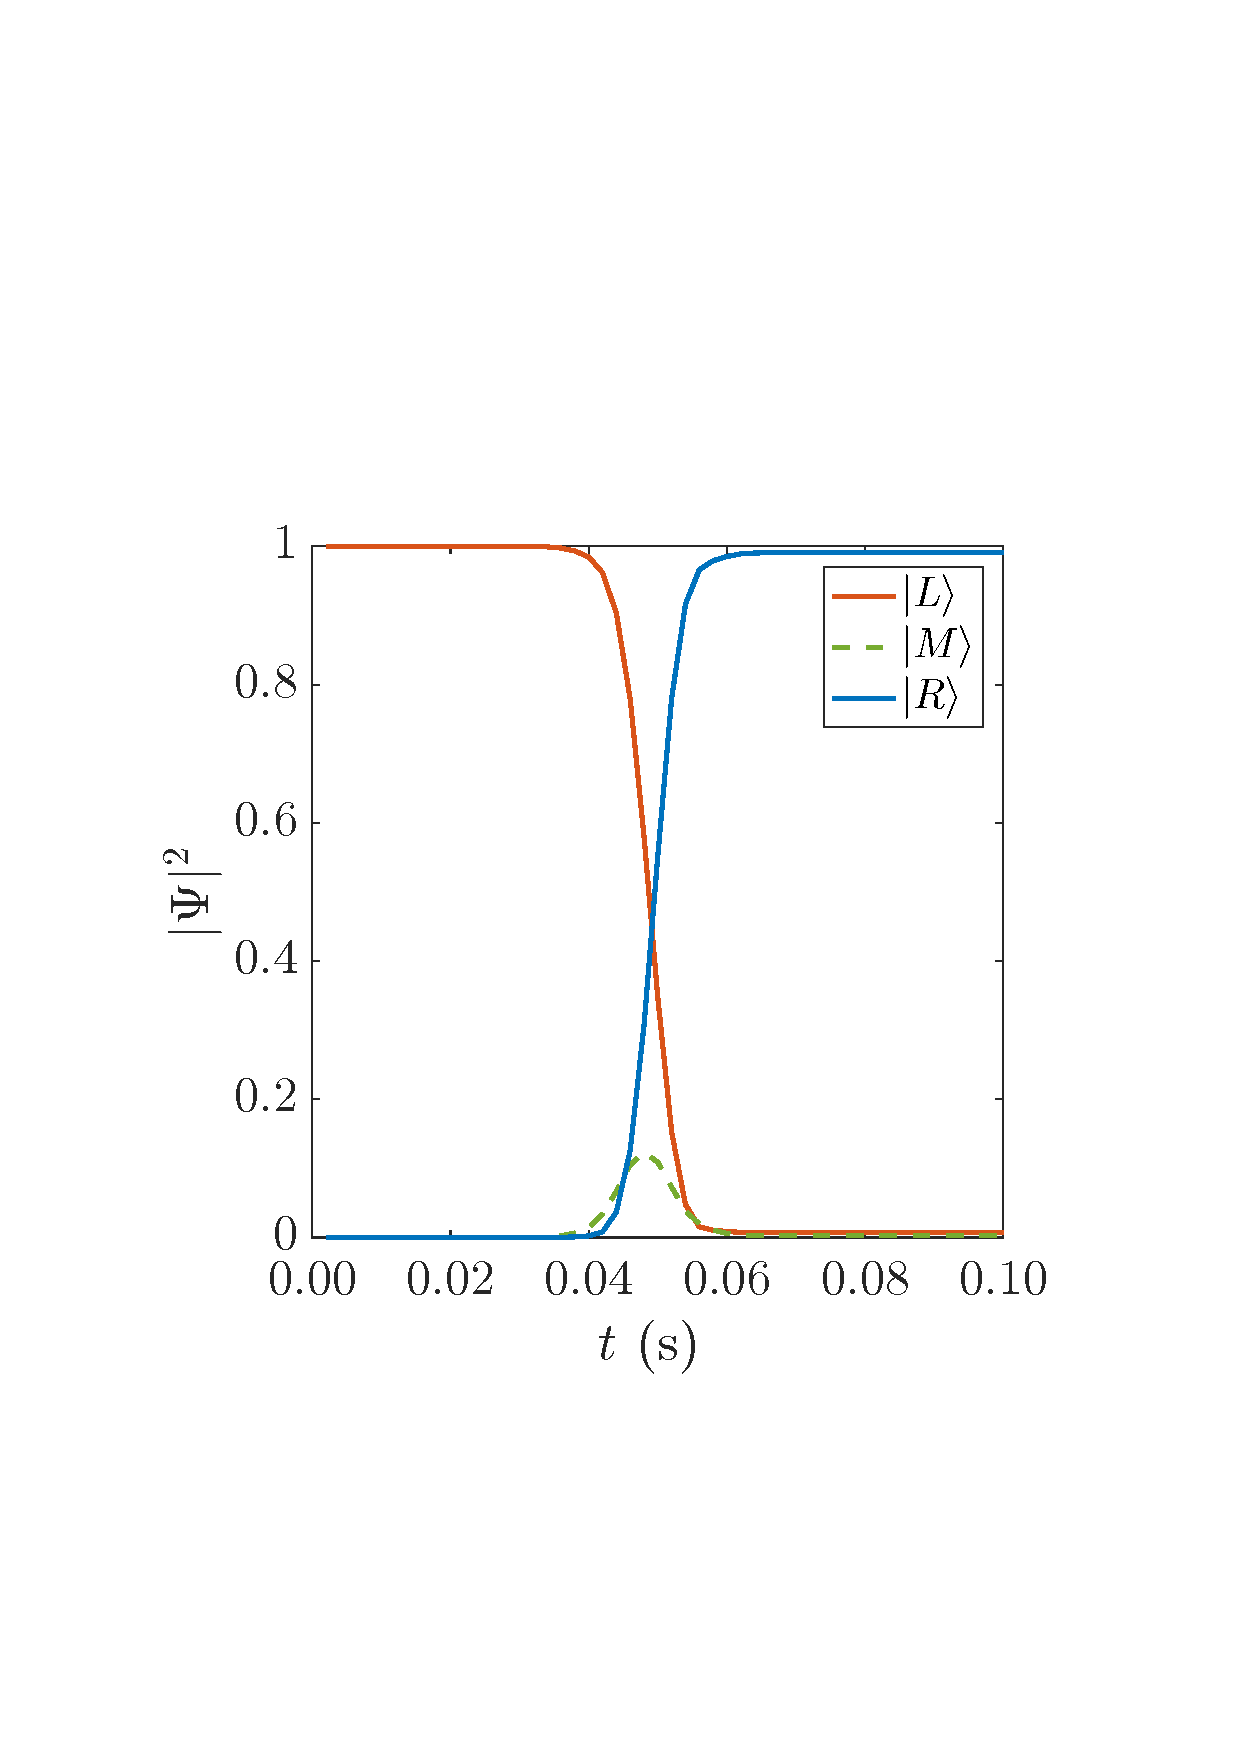
\includegraphics[width=0.47\textwidth]{ch3_numerics/STIRAP_CINT_POP}
  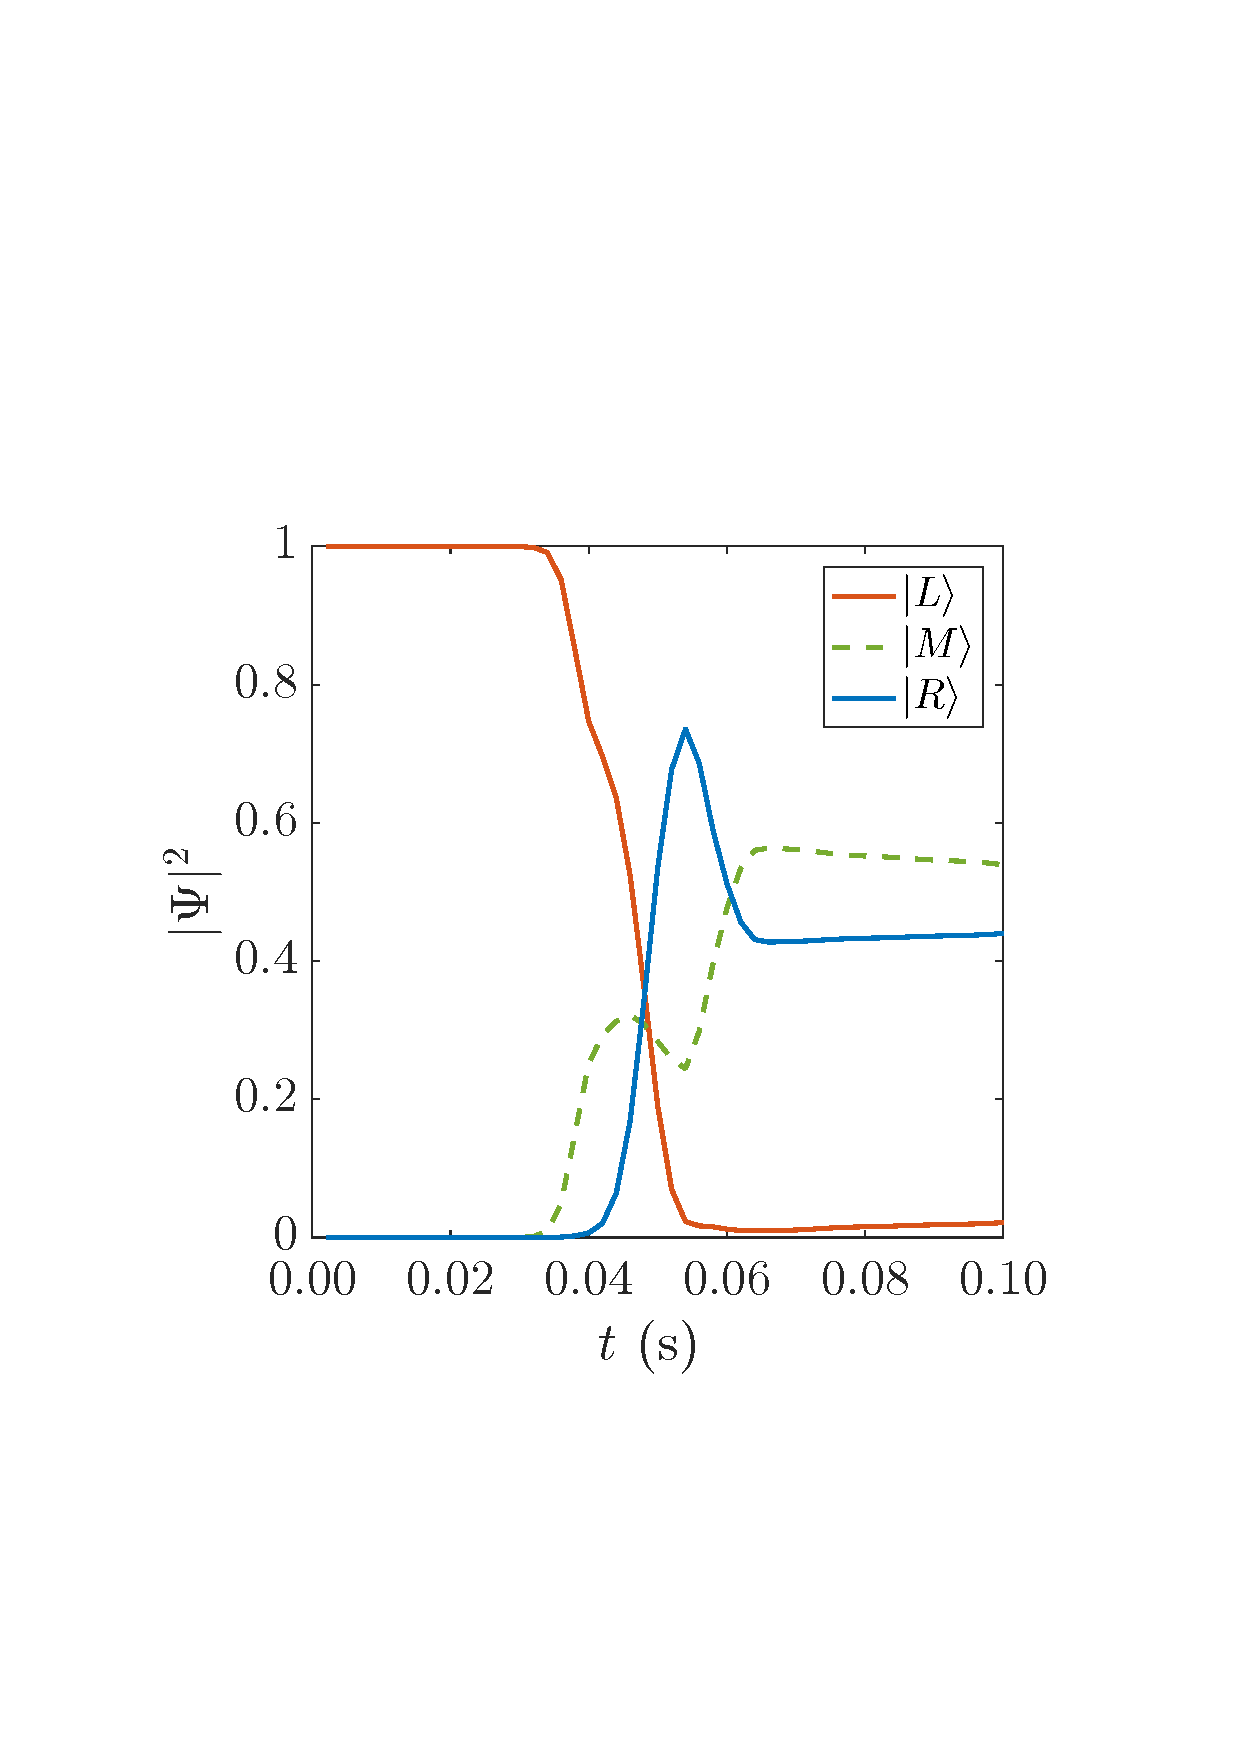
\includegraphics[width=0.47\textwidth]{ch3_numerics/STIRAP_INT_POP}
  \caption{pop}
  \label{fig:Populations}
\end{figure}

\begin{figure}[tb]
    \centering
  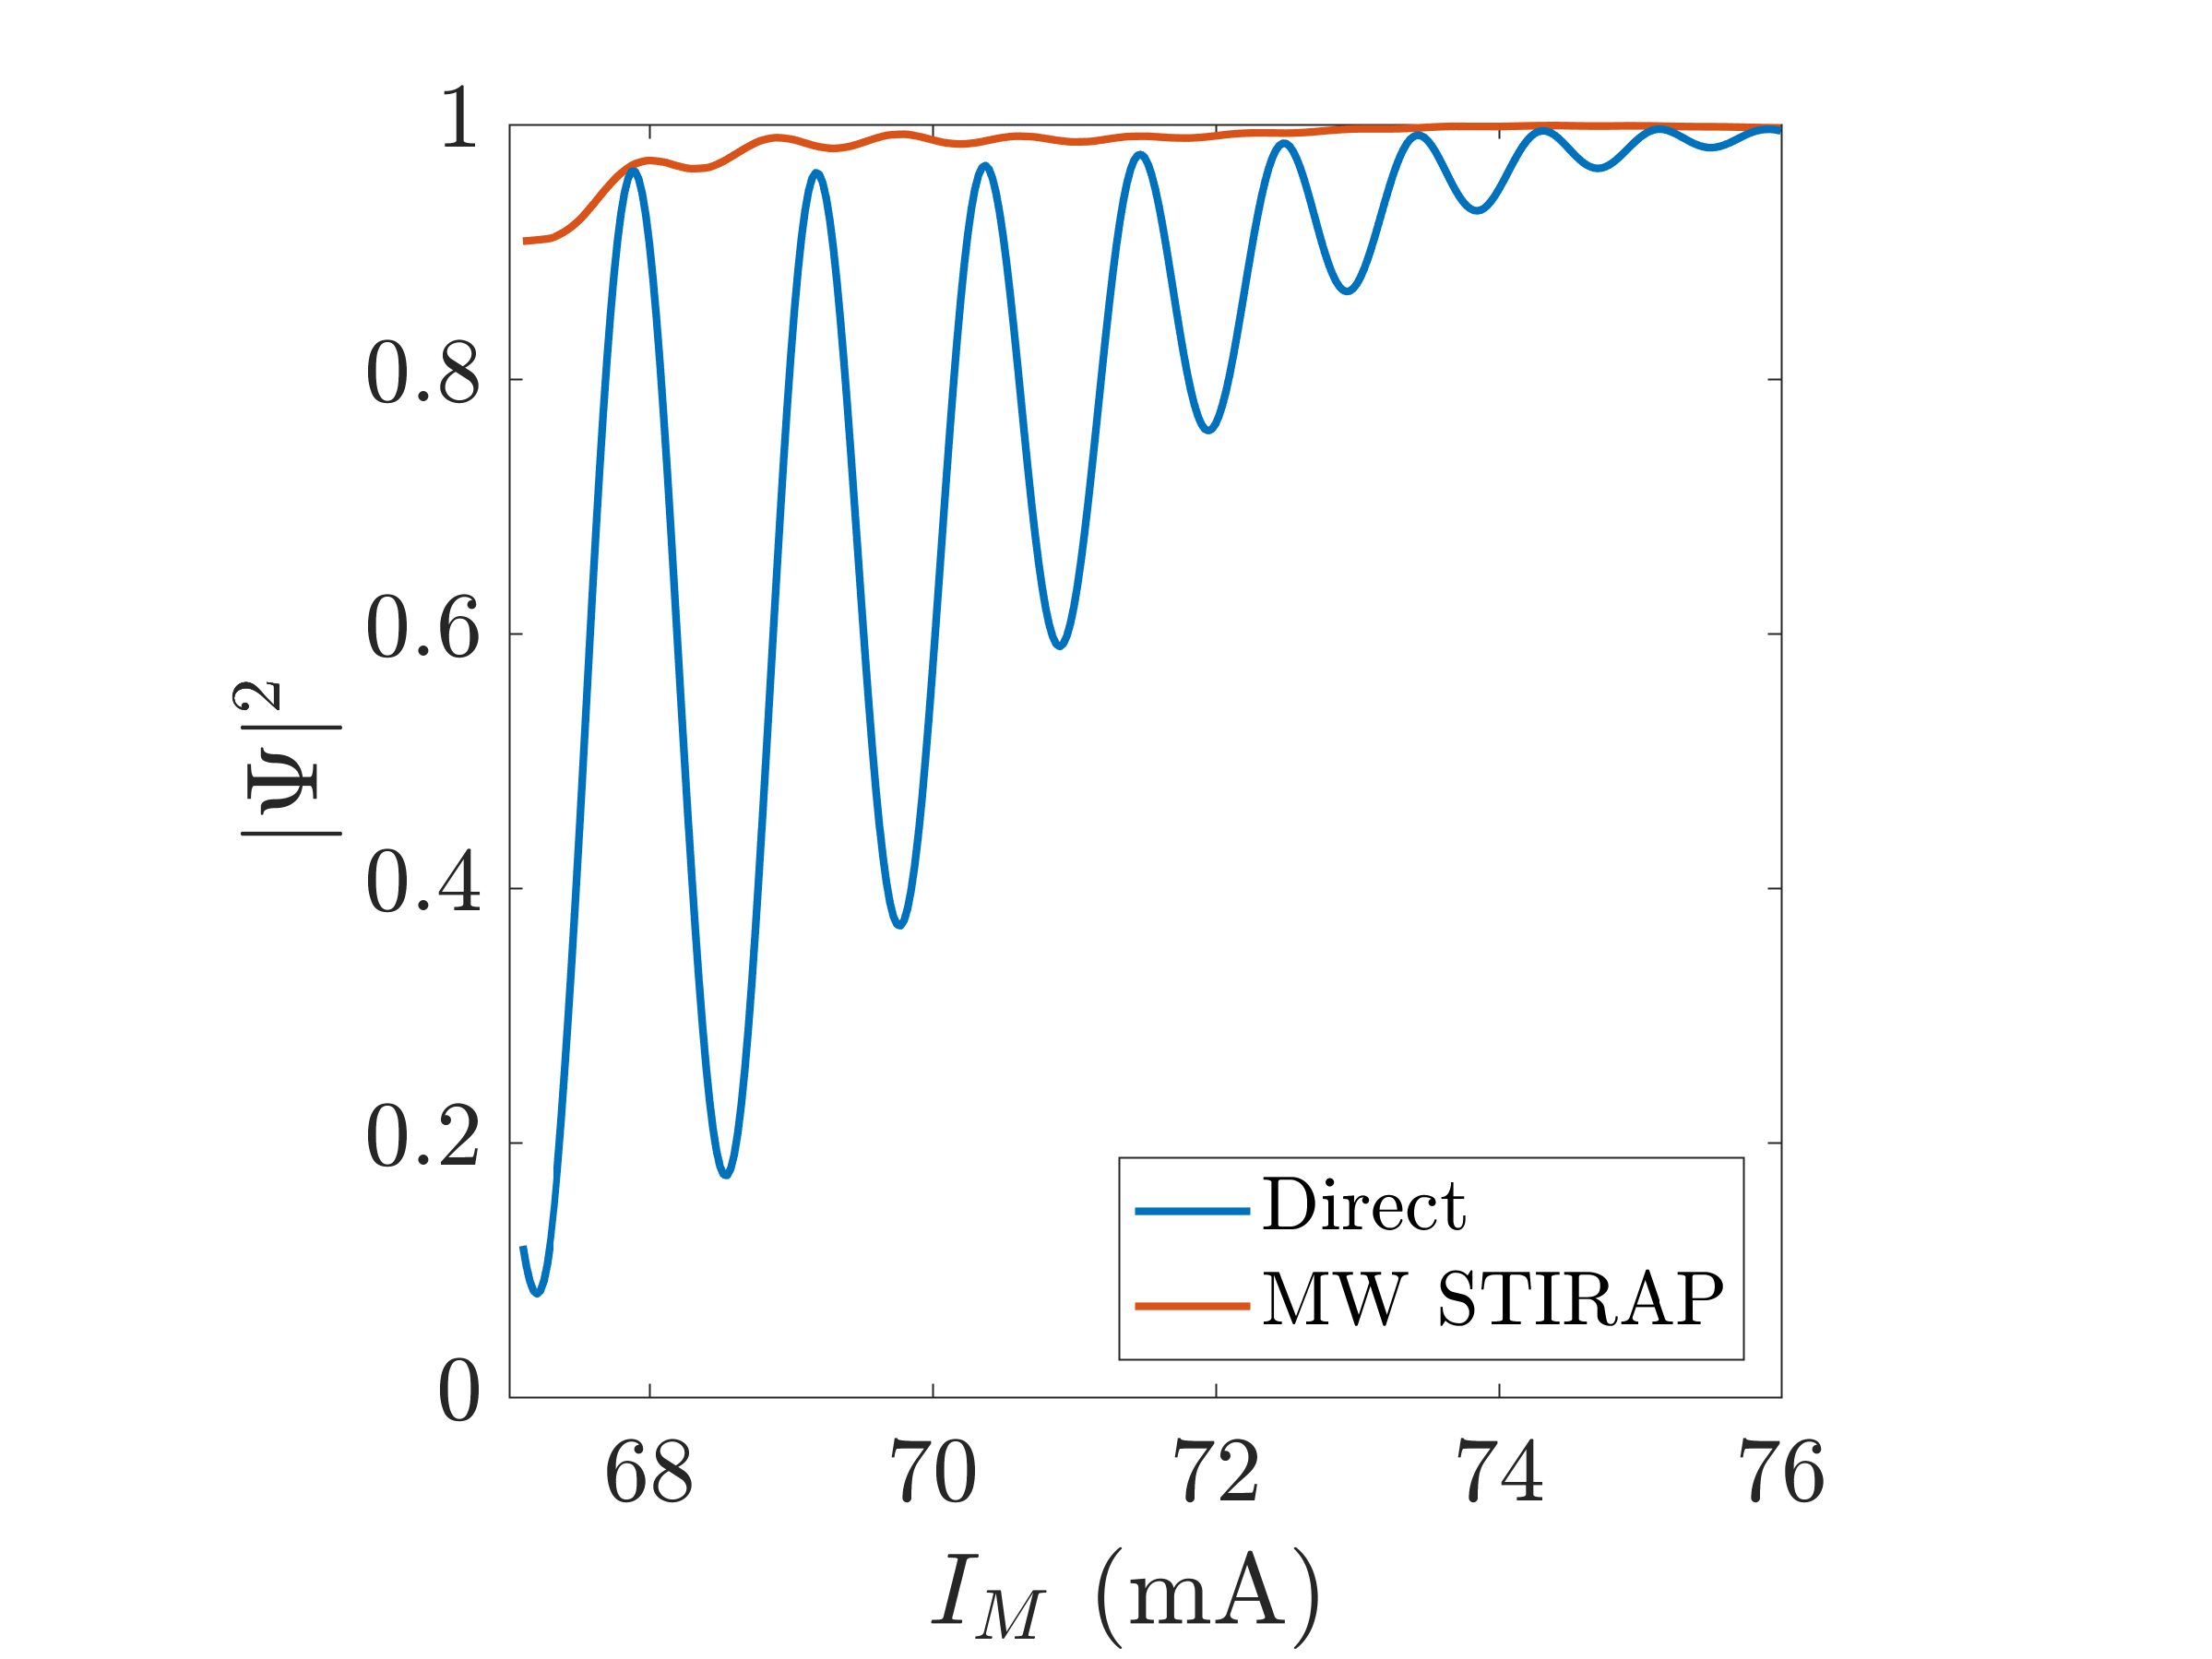
\includegraphics[width=0.85\textwidth]{ch3_numerics/DIRVSMWSTIRAP.png}
  \caption{pop}
  \label{fig:Populations}
\end{figure}
